% Created by tikzDevice version 0.10.1 on 2018-01-22 15:34:40
% !TEX encoding = UTF-8 Unicode
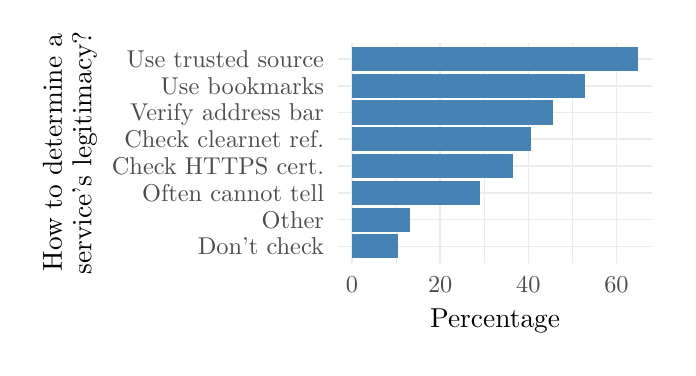
\begin{tikzpicture}[x=1pt,y=1pt]
\definecolor{fillColor}{RGB}{255,255,255}
\path[use as bounding box,fill=fillColor,fill opacity=0.00] (0,0) rectangle (231.26,115.63);
\begin{scope}
\path[clip] (112.04, 30.77) rectangle (225.76,110.13);
\definecolor{drawColor}{gray}{0.92}

\path[draw=drawColor,line width= 0.3pt,line join=round] (133.14, 30.77) --
	(133.14,110.13);

\path[draw=drawColor,line width= 0.3pt,line join=round] (164.99, 30.77) --
	(164.99,110.13);

\path[draw=drawColor,line width= 0.3pt,line join=round] (196.84, 30.77) --
	(196.84,110.13);

\path[draw=drawColor,line width= 0.6pt,line join=round] (112.04, 36.58) --
	(225.76, 36.58);

\path[draw=drawColor,line width= 0.6pt,line join=round] (112.04, 46.26) --
	(225.76, 46.26);

\path[draw=drawColor,line width= 0.6pt,line join=round] (112.04, 55.94) --
	(225.76, 55.94);

\path[draw=drawColor,line width= 0.6pt,line join=round] (112.04, 65.61) --
	(225.76, 65.61);

\path[draw=drawColor,line width= 0.6pt,line join=round] (112.04, 75.29) --
	(225.76, 75.29);

\path[draw=drawColor,line width= 0.6pt,line join=round] (112.04, 84.97) --
	(225.76, 84.97);

\path[draw=drawColor,line width= 0.6pt,line join=round] (112.04, 94.65) --
	(225.76, 94.65);

\path[draw=drawColor,line width= 0.6pt,line join=round] (112.04,104.33) --
	(225.76,104.33);

\path[draw=drawColor,line width= 0.6pt,line join=round] (117.21, 30.77) --
	(117.21,110.13);

\path[draw=drawColor,line width= 0.6pt,line join=round] (149.06, 30.77) --
	(149.06,110.13);

\path[draw=drawColor,line width= 0.6pt,line join=round] (180.91, 30.77) --
	(180.91,110.13);

\path[draw=drawColor,line width= 0.6pt,line join=round] (212.76, 30.77) --
	(212.76,110.13);
\definecolor{fillColor}{RGB}{70,130,180}

\path[fill=fillColor] (117.21, 32.22) rectangle (133.89, 40.93);

\path[fill=fillColor] (117.21, 41.90) rectangle (138.20, 50.61);

\path[fill=fillColor] (117.21, 51.58) rectangle (163.51, 60.29);

\path[fill=fillColor] (117.21, 61.26) rectangle (175.23, 69.97);

\path[fill=fillColor] (117.21, 70.94) rectangle (181.71, 79.65);

\path[fill=fillColor] (117.21, 80.61) rectangle (189.73, 89.32);

\path[fill=fillColor] (117.21, 90.29) rectangle (201.47, 99.00);

\path[fill=fillColor] (117.21, 99.97) rectangle (220.59,108.68);
\end{scope}
\begin{scope}
\path[clip] (  0.00,  0.00) rectangle (231.26,115.63);
\definecolor{drawColor}{gray}{0.30}

\node[text=drawColor,anchor=base east,inner sep=0pt, outer sep=0pt, scale=  0.88] at (107.09, 33.55) {Don't check};

\node[text=drawColor,anchor=base east,inner sep=0pt, outer sep=0pt, scale=  0.88] at (107.09, 43.23) {Other};

\node[text=drawColor,anchor=base east,inner sep=0pt, outer sep=0pt, scale=  0.88] at (107.09, 52.91) {Often cannot tell};

\node[text=drawColor,anchor=base east,inner sep=0pt, outer sep=0pt, scale=  0.88] at (107.09, 62.58) {Check HTTPS cert.};

\node[text=drawColor,anchor=base east,inner sep=0pt, outer sep=0pt, scale=  0.88] at (107.09, 72.26) {Check clearnet ref.};

\node[text=drawColor,anchor=base east,inner sep=0pt, outer sep=0pt, scale=  0.88] at (107.09, 81.94) {Verify address bar};

\node[text=drawColor,anchor=base east,inner sep=0pt, outer sep=0pt, scale=  0.88] at (107.09, 91.62) {Use bookmarks};

\node[text=drawColor,anchor=base east,inner sep=0pt, outer sep=0pt, scale=  0.88] at (107.09,101.29) {Use trusted source};
\end{scope}
\begin{scope}
\path[clip] (  0.00,  0.00) rectangle (231.26,115.63);
\definecolor{drawColor}{gray}{0.30}

\node[text=drawColor,anchor=base,inner sep=0pt, outer sep=0pt, scale=  0.88] at (117.21, 19.76) {0};

\node[text=drawColor,anchor=base,inner sep=0pt, outer sep=0pt, scale=  0.88] at (149.06, 19.76) {20};

\node[text=drawColor,anchor=base,inner sep=0pt, outer sep=0pt, scale=  0.88] at (180.91, 19.76) {40};

\node[text=drawColor,anchor=base,inner sep=0pt, outer sep=0pt, scale=  0.88] at (212.76, 19.76) {60};
\end{scope}
\begin{scope}
\path[clip] (  0.00,  0.00) rectangle (231.26,115.63);
\definecolor{drawColor}{RGB}{0,0,0}

\node[text=drawColor,anchor=base,inner sep=0pt, outer sep=0pt, scale=  0.99] at (168.90,  7.44) {Percentage};
\end{scope}
\begin{scope}
\path[clip] (  0.00,  0.00) rectangle (231.26,115.63);
\definecolor{drawColor}{RGB}{0,0,0}

\node[text=drawColor,rotate= 90.00,anchor=base,inner sep=0pt, outer sep=0pt, scale=  0.99] at ( 12.32, 70.45) {How to determine a};

\node[text=drawColor,rotate= 90.00,anchor=base,inner sep=0pt, outer sep=0pt, scale=  0.99] at ( 23.01, 70.45) {service's legitimacy?};
\end{scope}
\end{tikzpicture}
